\documentclass[aspectratio=169, table, 12pt]{beamer}

% Preamble bersama seluruh slide mata kuliah ini.
% Dipanggil dari slides/sessionXX/sessionXX.tex tepat sesudah baris
% \documentclass[aspectratio=169, table, 12pt]{beamer}
% Paket tambahan yang hanya dibutuhkan satu sesi ditulis di berkas sesi itu.

\usepackage{colortbl}
\usepackage{xcolor}
\usepackage{listings}
\usepackage{tabularx}
\usepackage{booktabs}
\usepackage{tikz}
\usepackage{pgfplots}
\pgfplotsset{compat=1.18}
\usetikzlibrary{arrows.meta, positioning, calc, fit, shapes.geometric,
	shapes.multipart, backgrounds, matrix, chains, trees}

\makeatletter
\def\input@path{{../theme/}}
\makeatother
\graphicspath{{../theme/}{../../figures/}}
\usetheme{Pradita}

\definecolor{praditagreen}{RGB}{37, 113, 71}

% Tema membuat garis tabel berwarna putih. Dikembalikan agar tabel terbaca.
\arrayrulecolor{black}
\setlength{\arrayrulewidth}{0.5pt}

\lstdefinelanguage{yaml}{
	basicstyle=\ttfamily\scriptsize,
	keywordstyle=\color{blue}\bfseries,
	commentstyle=\color{gray}\itshape,
	stringstyle=\color{red},
	showstringspaces=false,
	breaklines=true,
	frame=lines,
	numbers=none,
	backgroundcolor=\color{lightgray!10},
	tabsize=2,
	morecomment=[l]{\#}
}

\lstdefinelanguage{json}{
	basicstyle=\ttfamily\scriptsize,
	stringstyle=\color{red},
	commentstyle=\color{gray},
	breaklines=true,
	showstringspaces=false,
	tabsize=2,
	numbers=none,
	frame=lines,
	backgroundcolor=\color{lightgray!10},
	string=[s]{"}{"}
}

\lstdefinelanguage{bash}{
	keywords={},
	basicstyle=\ttfamily\scriptsize,
	ndkeywords={docker, kubectl, helm, curl, git, terraform},
	ndkeywordstyle=\color{purple}\bfseries,
	sensitive=true,
	commentstyle=\color{gray},
	numbers=none,
	breaklines=true,
	frame=lines,
	backgroundcolor=\color{lightgray!10},
	tabsize=2,
	comment=[l]{\#},
	showstringspaces=false
}

\lstdefinelanguage{http}{
	keywords={GET, POST, PUT, PATCH, DELETE, HEAD, OPTIONS, HTTP},
	basicstyle=\ttfamily\scriptsize,
	keywordstyle=\color{blue}\bfseries,
	sensitive=true,
	numbers=none,
	breaklines=true,
	frame=lines,
	backgroundcolor=\color{lightgray!10},
	tabsize=2,
	showstringspaces=false
}

\subtitle{IT40713 · Cloud-Native \& Microservices Architecture}
\author{\textbf{Alfa Yohannis}}


% Kolom X rata kiri untuk tabel yang sempit.
\newcolumntype{Y}{>{\raggedright\arraybackslash}X}

\title{\Huge Adopsi Cloud dan\\ \vspace{10pt} Strategi Migrasi 7R}

\begin{document}

\frame{\titlepage}

\begin{frame}
  \frametitle{Isi Pertemuan}
  \vspace{10pt}
  \begin{columns}[t]
    \column{0.5\textwidth}
    {\small\tableofcontents[sections={1-4}]}

    \column{0.5\textwidth}
    {\small\tableofcontents[sections={5-8}]}
  \end{columns}
\end{frame}

\begin{frame}{\hfill}
  \centering
  \LARGE{\textbf{Dari 46 aplikasi hasil akuisisi,\\mana yang dipindah lebih dulu,\\dan
  apakah organisasinya siap?}}
\end{frame}

\section{Tujuan dan Kerangka Bahasan}

\begin{frame}{\hfill}
  \centering
  \Huge{\textbf{Tujuan dan Kerangka Bahasan}}
\end{frame}

\begin{frame}{Tujuan Pembelajaran}
  \vspace{6pt}
  \begin{itemize}
    \item Membandingkan struktur kerangka adopsi \textit{cloud} dari AWS (Amazon Web
          Services), Microsoft, dan Google.
    \item Menilai kesiapan organisasi dengan enam perspektif AWS CAF.
    \item Memberi usulan strategi 7R yang beralasan untuk setiap aplikasi dalam
          portofolio.
  \end{itemize}
\end{frame}

\begin{frame}{Masalah yang Dijawab Pertemuan Ini}
  \begin{itemize}
    \item Misalkan inventaris pertama Medikara Health mencatat 46 aplikasi.
    \item Bab 2 mengusulkan model \textit{hybrid} dan menunda keputusan ERP keuangan.
    \item Bab 3 menghitung biaya per kunjungan pasien.
    \item Migrasi yang hanya digerakkan divisi TI sering gagal: pengguna tidak dilatih,
          anggaran tanpa pemilik, kontrol akses lemah ikut pindah.
    \item Urutan bahasan: kerangka, kesiapan, inventaris, 7R, \textit{landing zone}.
  \end{itemize}
\end{frame}

\begin{frame}{{\Large Diagram Konsep Bab 4}}
  \centering
  {\small\bfseries Kesiapan dan fondasi mendahului gelombang migrasi}\par\medskip
  \adjustbox{width=0.96\textwidth,height=0.7\textheight,keepaspectratio}{%
    % Diagram konsep Bab 4: Kesiapan dan fondasi mendahului gelombang migrasi.
% Dibangkitkan tools/render-diagrams.py dari figures/chapter-diagrams.json;
% ubah data JSON lalu jalankan ulang skrip, jangan sunting berkas ini langsung.
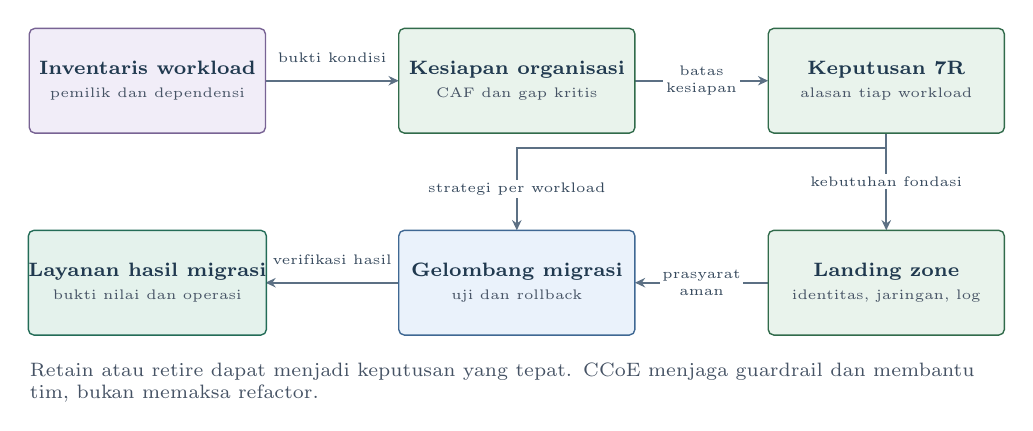
\begin{tikzpicture}[
  x=0.92cm, y=0.95cm,
  kotak konsep/.style={draw, line width=0.5pt, rounded corners=2pt,
    align=center, minimum width=2.999cm,
    minimum height=1.330cm, inner sep=0pt, font=\scriptsize,
    text=konsepJudul},
  peran actor/.style={kotak konsep, fill=konsepIsiActor, draw=konsepGarisActor},
  peran service/.style={kotak konsep, fill=konsepIsiService, draw=konsepGarisService},
  peran control/.style={kotak konsep, fill=konsepIsiControl, draw=konsepGarisControl},
  peran data/.style={kotak konsep, fill=konsepIsiData, draw=konsepGarisData},
  peran outcome/.style={kotak konsep, fill=konsepIsiOutcome, draw=konsepGarisOutcome},
  peran risk/.style={kotak konsep, fill=konsepIsiRisk, draw=konsepGarisRisk},
  panah konsep/.style={-{Stealth[length=1.3mm, width=1.2mm]}, line width=0.6pt,
    draw=konsepPanah},
  panah putus/.style={panah konsep, draw=konsepPanahPutus,
    dash pattern=on 2.5pt off 1.5pt},
  label panah/.style={font=\tiny, align=center, fill=white,
    inner sep=1pt, text=konsepLabel},
  catatan/.style={font=\scriptsize, align=left, anchor=north west,
    inner sep=0pt, text width=12.383cm, text=konsepTeks,
    execute at begin node={\hyphenpenalty=10000\hbadness=10000\relax}},
]
  \definecolor{konsepIsiActor}{HTML}{EEF1F6}
  \definecolor{konsepGarisActor}{HTML}{50627D}
  \definecolor{konsepIsiService}{HTML}{EAF2FB}
  \definecolor{konsepGarisService}{HTML}{3F6893}
  \definecolor{konsepIsiControl}{HTML}{E9F3EC}
  \definecolor{konsepGarisControl}{HTML}{316B4B}
  \definecolor{konsepIsiData}{HTML}{F1EDF8}
  \definecolor{konsepGarisData}{HTML}{786394}
  \definecolor{konsepIsiOutcome}{HTML}{E4F2EC}
  \definecolor{konsepGarisOutcome}{HTML}{236C57}
  \definecolor{konsepIsiRisk}{HTML}{FCEDE7}
  \definecolor{konsepGarisRisk}{HTML}{B36947}
  \definecolor{konsepJudul}{HTML}{20394F}
  \definecolor{konsepTeks}{HTML}{455264}
  \definecolor{konsepLabel}{HTML}{35485C}
  \definecolor{konsepPanah}{HTML}{5C7084}
  \definecolor{konsepPanahPutus}{HTML}{A15D40}
  % Panah dan label lebih dahulu; kotak menutupi sisa latar label.
  \draw[panah konsep] (0.93,0) -- (2.77,0);
  \draw[panah konsep] (6.03,0) -- (7.87,0);
  \draw[panah konsep] (9.5,-0.7) -- (9.5,-2);
  \draw[panah konsep] (7.87,-2.7) -- (6.03,-2.7);
  \draw[panah konsep] (9.5,-0.7) -- (9.5,-0.9) -- (4.4,-0.9) -- (4.4,-2);
  \draw[panah konsep] (2.77,-2.7) -- (0.93,-2.7);
  \node[label panah] at (1.85,0.31) {bukti kondisi};
  \node[label panah] at (6.95,0) {batas\\kesiapan};
  \node[label panah] at (9.5,-1.35) {kebutuhan fondasi};
  \node[label panah] at (6.95,-2.7) {prasyarat\\aman};
  \node[label panah] at (4.4,-1.45) {strategi per workload};
  \node[label panah] at (1.85,-2.39) {verifikasi hasil};
  \node[peran data] (invent) at (-0.7,0)
    {\textbf{Inventaris workload}\\[0.5pt]{\tiny\color{konsepTeks}pemilik dan dependensi}};
  \node[peran control] (siap) at (4.4,0)
    {\textbf{Kesiapan organisasi}\\[0.5pt]{\tiny\color{konsepTeks}CAF dan gap kritis}};
  \node[peran control] (r) at (9.5,0)
    {\textbf{Keputusan 7R}\\[0.5pt]{\tiny\color{konsepTeks}alasan tiap workload}};
  \node[peran outcome] (ukur) at (-0.7,-2.7)
    {\textbf{Layanan hasil migrasi}\\[0.5pt]{\tiny\color{konsepTeks}bukti nilai dan operasi}};
  \node[peran service] (migrasi) at (4.4,-2.7)
    {\textbf{Gelombang migrasi}\\[0.5pt]{\tiny\color{konsepTeks}uji dan rollback}};
  \node[peran control] (zona) at (9.5,-2.7)
    {\textbf{Landing zone}\\[0.5pt]{\tiny\color{konsepTeks}identitas, jaringan, log}};
  \node[catatan] at (-2.33,-3.77)
    {Retain atau retire dapat menjadi keputusan yang tepat. CCoE menjaga guardrail dan membantu tim, bukan memaksa refactor.};
\end{tikzpicture}
}
\end{frame}

\section{Tiga Kerangka Adopsi Cloud}

\begin{frame}{\hfill}
  \centering
  \Huge{\textbf{Tiga Kerangka Adopsi Cloud}}
\end{frame}

\begin{frame}{Apa Itu Kerangka Adopsi Cloud}
  \begin{itemize}
    \item CAF (\textit{Cloud Adoption Framework}): panduan, praktik, dan alat bantu untuk
          adopsi \textit{cloud} di tingkat organisasi.
    \item Menurut AWS: memprioritaskan peluang, menilai kesiapan, memperbarui peta jalan
          secara bertahap.
    \item Analogi: buku panduan jasa pindahan kantor. Judul babnya beda, isinya mirip.
    \item Misalkan Bekasi memindah jadwal kamar operasi tanpa melatih 40 perawat: celah
          orang.
    \item Misalkan Depok membuka akun sendiri, Rp18 juta per bulan tanpa pemilik: celah
          tata kelola.
  \end{itemize}
\end{frame}

\begin{frame}{AWS CAF: Enam Perspektif, Empat Domain, Empat Fase}
  \centering
  \eadiagram{../../figures/ch04-struktur-aws-caf.tex}
\end{frame}

\begin{frame}{Microsoft CAF dan Google Cloud Adoption Framework}
  \begin{columns}[t]
    \column{0.48\textwidth}
    \textbf{Microsoft CAF (pembaruan Agustus 2026)}
    \begin{itemize}
      \item Tujuh fase: Strategy, Plan, Ready, Adopt, Govern, Secure, Manage.
      \item Ready menyiapkan \textit{landing zone}.
      \item Ada skenario kedaulatan data.
      \item Mudah dijadikan paket kerja.
    \end{itemize}

    \column{0.48\textwidth}
    \textbf{Google Cloud Adoption Framework}
    \begin{itemize}
      \item Empat tema: Learn, Lead, Scale, Secure.
      \item Tiga fase: \textit{tactical}, \textit{strategic},
            \textit{transformational}.
      \item Dibaca lewat orang, proses, dan teknologi.
      \item Mudah dikomunikasikan ke direksi.
    \end{itemize}
  \end{columns}
\end{frame}

\begin{frame}{Perbandingan Tiga Kerangka}
  \footnotesize
  \begin{tabularx}{\textwidth}{>{\raggedright\arraybackslash}p{2.6cm}YYY}
    \hline
    \textbf{Aspek} & \textbf{AWS CAF} & \textbf{Microsoft CAF} & \textbf{Google CAF} \\
    \hline
    Unit utama & Enam perspektif & Tujuh fase & Empat tema \\
    \hline
    Paling membantu menjawab & Siapa memiliki kemampuan apa? & Pekerjaan apa lebih dulu?
      & Sudah semampu apa sekarang? \\
    \hline
    Kekuatan & Memetakan pemangku kepentingan & Paket kerja proyek & Tingkat kematangan
      \\
    \hline
    Kelemahan bila sendirian & Tanpa urutan kerja rinci & Terbaca sebagai urusan TI
      saja & Kurang rinci per kemampuan \\
    \hline
  \end{tabularx}

  \vspace{8pt}
  Bab ini memakai enam perspektif AWS CAF untuk menilai kesiapan.
\end{frame}

\begin{frame}{Dua Hal yang Sering Tertukar}
  \begin{itemize}
    \item Kerangka adopsi (CAF) menilai kesiapan organisasi dan mengatur perjalanan
          adopsi.
    \item Kerangka arsitektur (Well-Architected, enam pilar) menilai mutu rancangan satu
          \textit{workload}.
    \item "Apakah tim keamanan sudah siap?" milik CAF.
    \item "Apakah SIMRS punya cadangan di dua zona?" milik kerangka arsitektur.
  \end{itemize}
\end{frame}

\section{Penilaian Kesiapan}

\begin{frame}{\hfill}
  \centering
  \Huge{\textbf{Penilaian Kesiapan dengan\\Enam Perspektif}}
\end{frame}

\begin{frame}{Enam Perspektif dan Pemangku Kepentingannya}
  \scriptsize
  \begin{tabularx}{\textwidth}{>{\raggedright\arraybackslash}p{2cm}Y
      >{\raggedright\arraybackslash}p{4.4cm}}
    \hline
    \textbf{Perspektif} & \textbf{Pertanyaan kunci} & \textbf{Pemangku kepentingan} \\
    \hline
    Business & Hasil bisnis apa, berapa angkanya, siapa pemilik manfaat? & Direktur
      utama, keuangan, operasional \\
    \hline
    People & Keterampilan, budaya, struktur tim apa yang berubah? & Kepala TI, kepala
      sumber daya manusia \\
    \hline
    Governance & Siapa memutuskan; bagaimana anggaran dan risiko dikendalikan? & Direktur
      keuangan, manajemen risiko \\
    \hline
    Platform & Lingkungan apa yang dibangun dan disiapkan berulang? & Arsitek,
      \textit{engineer} infrastruktur \\
    \hline
    Security & Bagaimana data dan \textit{workload} dijaga? & Keamanan informasi,
      kepatuhan, audit internal \\
    \hline
    Operations & Bagaimana layanan dipantau, dipulihkan, diubah? & Kepala operasional TI
      \\
    \hline
  \end{tabularx}
\end{frame}

\begin{frame}{Memberi Skor tanpa Terjebak Formalitas}
  \begin{itemize}
    \item Skor 1 sampai 5: belum ada, informal, terdokumentasi sebagian, konsisten dan
          diukur, diperbaiki berdasarkan data.
    \item Setiap skor wajib disertai bukti. Skor tanpa bukti dicatat 1.
    \item Penilai bukan pemilik proses yang dinilai.
    \item Keputusan dibaca dari skor terendah, bukan rata-rata.
    \item Setiap celah punya pemilik, rencana, dan tanggal tinjau ulang.
  \end{itemize}
\end{frame}

\begin{frame}{Pemeriksaan Kesehatan, Bukan Audit}
  \begin{itemize}
    \item Analogi: lima hasil normal dan satu kadar gula jauh di atas batas tetap perlu
          ditangani sekarang.
    \item Audit memeriksa kepatuhan pada aturan dan menghasilkan temuan.
    \item Penilaian kesiapan memeriksa kemampuan untuk perubahan dan menghasilkan
          rencana.
    \item Misalkan rata-rata 3,4 tetapi Security 1,7 karena akun administrator dipakai 9
          orang: belum siap.
  \end{itemize}
\end{frame}

\begin{frame}{Kasus Medikara: Profil Kesiapan (Angka Rekaan)}
  \begin{columns}[c]
    \column{0.55\textwidth}
    \centering
    \resizebox{!}{0.62\textheight}{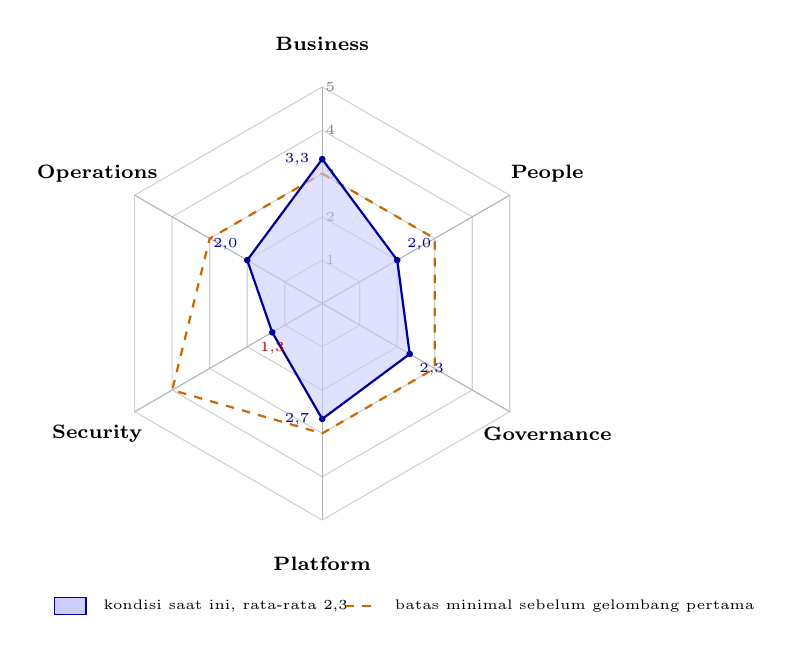
\begin{tikzpicture}[font=\scriptsize]
  % Satu satuan skor sama dengan 0,55 cm. Skala 1 sampai 5.
  \foreach \skor in {1,...,5} {
    \draw[gray!35] (90:{\skor*0.55}) -- (30:{\skor*0.55}) -- (-30:{\skor*0.55})
      -- (-90:{\skor*0.55}) -- (-150:{\skor*0.55}) -- (150:{\skor*0.55}) -- cycle;
    \node[gray, font=\tiny, anchor=west, inner sep=1pt] at (90:{\skor*0.55}) {\skor};
  }

  % Enam sumbu perspektif. Sisi kanan bisnis, sisi kiri teknis.
  \foreach \sudut/\nama in {90/Business, 30/People, -30/Governance,
    -90/Platform, -150/Security, 150/Operations} {
    \draw[gray!60] (0,0) -- (\sudut:2.75);
    \node[font=\scriptsize\bfseries] at (\sudut:3.3) {\nama};
  }

  % Batas minimal sebelum gelombang pertama: 3, kecuali Security 4.
  \draw[thick, dashed, orange!80!black] (90:1.65) -- (30:1.65) -- (-30:1.65)
    -- (-90:1.65) -- (-150:2.2) -- (150:1.65) -- cycle;

  % Kondisi saat ini, rata-rata tiga pertanyaan per perspektif.
  \draw[thick, draw=blue!60!black, fill=blue!20, fill opacity=0.6]
    (90:1.833) -- (30:1.1) -- (-30:1.283) -- (-90:1.467) -- (-150:0.733)
    -- (150:1.1) -- cycle;
  \foreach \sudut/\jarak in {90/1.833, 30/1.1, -30/1.283, -90/1.467,
    -150/0.733, 150/1.1} {
    \fill[blue!60!black] (\sudut:\jarak) circle (1.2pt);
  }
  \node[font=\tiny, blue!60!black, anchor=east] at (90:1.833) {3,3\,};
  \node[font=\tiny, blue!60!black, anchor=south west] at (30:1.1) {2,0};
  \node[font=\tiny, blue!60!black, anchor=north west] at (-30:1.283) {2,3};
  \node[font=\tiny, blue!60!black, anchor=east] at (-90:1.467) {2,7\,};
  \node[font=\tiny, red!70!black, anchor=north] at (-150:0.733) {1,3};
  \node[font=\tiny, blue!60!black, anchor=south east] at (150:1.1) {2,0};

  % Keterangan.
  \fill[blue!20, draw=blue!60!black] (-3.4,-3.95) rectangle ++(0.4,0.22);
  \node[anchor=west, font=\tiny] at (-2.9,-3.84) {kondisi saat ini, rata-rata 2,3};
  \draw[thick, dashed, orange!80!black] (0.3,-3.84) -- ++(0.4,0);
  \node[anchor=west, font=\tiny] at (0.8,-3.84)
    {batas minimal sebelum gelombang pertama};
\end{tikzpicture}
}

    \column{0.43\textwidth}
    \footnotesize
    \begin{itemize}
      \item 52 staf TI di lima rumah sakit dan kantor pusat; 4 bersertifikat.
      \item 212 akun SIMRS mantan karyawan masih aktif.
      \item Vendor Medikara+ memakai akun bersama.
      \item Rata-rata 2,3; Business 3,3; Security 1,3.
    \end{itemize}
  \end{columns}
\end{frame}

\begin{frame}{Kasus Medikara: Dua Konsekuensi}
  \begin{itemize}
    \item Batas minimal: 3 untuk setiap perspektif, 4 untuk Security.
    \item Pertama, gelombang pertama ditunda sekitar enam bulan.
    \item Tiga celah terbesar: Security (selisih 2,7), Operations (1,0), People (1,0).
    \item Kedua, pekerjaan tanpa memindahkan data pasien tidak perlu menunggu.
    \item Aplikasi yang tidak dipakai dimatikan; inventaris dimulai sekarang.
  \end{itemize}
\end{frame}

\section{Inventaris dan Dependensi}

\begin{frame}{\hfill}
  \centering
  \Huge{\textbf{Inventaris Portofolio\\dan Dependensi}}
\end{frame}

\begin{frame}{Atribut Minimal Inventaris}
  \footnotesize
  \begin{tabularx}{\textwidth}{>{\raggedright\arraybackslash}p{3cm}YY}
    \hline
    \textbf{Atribut} & \textbf{Mengapa dibutuhkan} & \textbf{Contoh: aplikasi apotek} \\
    \hline
    Pemilik bisnis dan teknis & Siapa memutuskan, siapa mengerjakan & Kepala unit apotek;
      TI pusat \\
    \hline
    Pengguna dan kritikalitas & Siapa terdampak, urutan gelombang & 96 staf di 12
      apotek; sedang \\
    \hline
    Teknologi, kontrak & Dapat dipindah apa adanya? Kapan paling murah? & Desktop;
      dukungan berhenti akhir 2026 \\
    \hline
    Dependensi & Aplikasi yang harus pindah bersama & Baca stok langsung dari basis data
      SIMRS \\
    \hline
    Kondisi & Masalah yang sudah dirasakan & Stok sinkron tiap malam \\
    \hline
  \end{tabularx}
\end{frame}

\begin{frame}{Kabel di Balik Lemari}
  \begin{itemize}
    \item Analogi: lampu kamar anak ternyata menyala dari stopkontak kamar sebelah.
    \item Flexera 2020 (750 responden): memahami dependensi aplikasi adalah tantangan
          teratas migrasi.
    \item Sumber pencarian: wawancara, berkas konfigurasi, jadwal tugas malam, log
          jaringan.
    \item Setiap sumber hanya menangkap sebagian, jadi dipakai bersamaan.
  \end{itemize}
\end{frame}

\begin{frame}{Peta Dependensi di Sekitar SIMRS Jakarta (Rekaan)}
  \centering
  \eadiagram{../../figures/ch04-peta-dependensi.tex}
\end{frame}

\begin{frame}{Kelompok Pindah: Apa yang Terungkap}
  \begin{itemize}
    \item Kelompok pindah: aplikasi yang harus dipindah dalam gelombang yang sama.
    \item Apotek membaca basis data SIMRS sekitar 30.000 kali per bulan: pindah bersama,
          atau ganti dengan antarmuka resmi.
    \item Skrip malam 30 kali per bulan menyatukan kelompok SIMRS dan ERP keuangan.
    \item Sistem laboratorium terikat kabel ke alat analisis: alat fisik tidak ikut
          pindah.
    \item Prinsip arsitektur dan \textit{gap analysis}: dibahas rinci di IT40513.
  \end{itemize}
\end{frame}

\section{Strategi Migrasi 7R}

\begin{frame}{\hfill}
  \centering
  \Huge{\textbf{Strategi Migrasi 7R}}
\end{frame}

\begin{frame}{Tujuh R Menurut AWS Prescriptive Guidance}
  \scriptsize
  \begin{tabularx}{\textwidth}{>{\raggedright\arraybackslash}p{2cm}YY}
    \hline
    \textbf{Strategi} & \textbf{Yang terjadi} & \textbf{Kasus pemakaian umum} \\
    \hline
    Retire & Dimatikan atau diarsipkan & Pemakaian di bawah 5 persen; tanpa koneksi masuk
      90 hari \\
    \hline
    Retain & Tetap di tempat sementara & Aturan lokasi data, perangkat khusus, menunggu
      SaaS \\
    \hline
    Rehost & Dipindah tanpa perubahan & Banyak server dengan cepat \\
    \hline
    Relocate & Pindah di tingkat platform & Platform virtualisasi; antarakun \\
    \hline
    Repurchase & Diganti produk lain & Lisensi lama ke SaaS \\
    \hline
    Replatform & Pindah dengan sebagian optimasi & Basis data ke layanan terkelola \\
    \hline
    Refactor & Arsitektur dirancang ulang & Monolit menghambat rilis \\
    \hline
  \end{tabularx}
\end{frame}

\begin{frame}{Analogi dan Tiga Strategi yang Sering Tertukar}
  \begin{itemize}
    \item Pindah rumah: buang, titip, angkut, kontainer utuh, beli baru, ganti engsel,
          rancang ulang dapur.
    \item Rehost: server satu per satu ke mesin virtual, aplikasi tidak diubah.
    \item Relocate: sekumpulan server sekaligus di tingkat platform, atau pindah antarakun.
    \item Replatform: sebagian kecil cara jalan diubah, misalnya basis data ke layanan
          terkelola.
  \end{itemize}
\end{frame}

\begin{frame}{Mengapa Tidak Sekalian Refactor?}
  \begin{itemize}
    \item AWS: Refactor tidak dianjurkan untuk migrasi besar, karena modernisasi
          dilakukan selama migrasi.
    \item Paling rumit, paling mahal, sulit dikelola untuk banyak aplikasi.
    \item Anjuran: \textit{rehost}, \textit{relocate}, atau \textit{replatform} dulu,
          modernisasi sesudahnya.
    \item Konsekuensi pertama: masa membayar dua lingkungan menjadi pendek.
    \item Konsekuensi kedua: masalah rancangan ikut pindah, jadi "kemudian" butuh
          tanggal dan anggaran.
  \end{itemize}
\end{frame}

\begin{frame}{Urutan Pertanyaan untuk Usulan Awal}
  \centering
  \eadiagram{../../figures/ch04-pohon-7r.tex}
\end{frame}

\begin{frame}{Kasus Medikara: Usulan 7R Awal (Rekaan)}
  \scriptsize
  \begin{tabularx}{\textwidth}{>{\raggedright\arraybackslash}p{3.6cm}
      >{\raggedright\arraybackslash}p{2.2cm}Y}
    \hline
    \textbf{Aplikasi} & \textbf{Usulan} & \textbf{Alasan singkat} \\
    \hline
    SIMRS, lima versi & Diperdebatkan & Retain lalu Repurchase, atau Rehost ke Jakarta \\
    \hline
    ERP keuangan & Replatform & Basis data ke layanan terkelola; lisensi sampai 2028 \\
    \hline
    Medikara+ & Relocate & Keluar dari akun vendor; Refactor menyusul \\
    \hline
    Sistem laboratorium & Retain & Terikat kabel ke alat analisis \\
    \hline
    Aplikasi apotek & Repurchase & Dukungan vendor berhenti; SaaS memadai \\
    \hline
    Klaster virtualisasi, 14 aplikasi & Relocate & Pindah utuh di tingkat platform \\
    \hline
    Portal dokumen akreditasi & Rehost & Aplikasi sederhana di perangkat tua \\
    \hline
    Antrean lama Jakarta & Retire & Tanpa koneksi masuk 90 hari \\
    \hline
  \end{tabularx}
\end{frame}

\begin{frame}{Kasus Medikara: Sebaran 46 Aplikasi}
  \begin{itemize}
    \item Retire 6, Retain 5, Rehost 10, Relocate 15, Repurchase 3, Replatform 2,
          Refactor 0, diperdebatkan 5.
    \item Tidak ada Refactor pada gelombang pertama; Medikara+ menyusul mulai Bab 8.
    \item SIMRS: Retain lalu Repurchase sejalan dengan strategi, tetapi melatih sekitar
          2.900 staf.
    \item SIMRS: Rehost cepat mengatasi perangkat tua, tetapi lima versi tetap lima.
    \item Bab 7 mendiagnosis bentuk arsitektur; keputusan akhir ada di peta jalan Bab 14.
  \end{itemize}
\end{frame}

\section{Landing Zone dan CCoE}

\begin{frame}{\hfill}
  \centering
  \Huge{\textbf{Landing Zone dan\\Cloud Center of Excellence}}
\end{frame}

\begin{frame}{Landing Zone: Fondasi Sebelum Workload Datang}
  \begin{itemize}
    \item Lingkungan \textit{cloud} yang disiapkan sebelum \textit{workload} pertama
          datang.
    \item Microsoft CAF: fase Ready, beberapa area rancangan.
    \item Isi umum: struktur akun, identitas dan akses, jaringan, kebijakan keamanan,
          log terpusat, tag dan anggaran.
    \item Analogi: kawasan perumahan yang jalan, saluran, dan pos satpamnya sudah jadi.
    \item Misalkan sesudah 8 minggu: akun baru siap dalam 1 hari, bukan 3 minggu.
  \end{itemize}
\end{frame}

\begin{frame}{Landing Zone Rancangan Awal Medikara}
  \centering
  \eadiagram{../../figures/ch04-landing-zone.tex}
\end{frame}

\begin{frame}{Cloud Center of Excellence (CCoE)}
  \begin{itemize}
    \item Tim lintas fungsi: arsitek, keamanan, keuangan, operasi, wakil unit bisnis.
    \item Flexera 2020: 73 persen perusahaan besar punya tim \textit{cloud} pusat atau
          CCoE.
    \item CCoE bukan divisi TI baru yang mengerjakan seluruh migrasi.
    \item Menetapkan standar, menyediakan fondasi, mengajari tim lain.
    \item Aturan yang dijaga disebut \textit{guardrail}; dibahas di Bab 14.
  \end{itemize}
\end{frame}

\section{Aktivitas}

\begin{frame}{Aktivitas: Penilaian Kesiapan dan Portofolio 7R}
  \begin{enumerate}
    \item Isi \texttt{lembar-penilaian-kesiapan-caf.xlsx}: skor, bukti, pemilik jawaban.
    \item Tetapkan batas minimal, catat tiga celah terbesar.
    \item Inventaris aplikasi di \texttt{templat-inventaris-aplikasi.xlsx}.
    \item Beri usulan 7R dengan alasan satu kalimat
          (\texttt{panduan-keputusan-7r.md}).
    \item Tandai usulan yang diperdebatkan beserta dua pilihannya.
  \end{enumerate}
\end{frame}

\begin{frame}{Peran, Luaran, dan Kriteria}
  \begin{itemize}
    \item Non-teknis memimpin Business, People, Governance; teknis memimpin Platform,
          Security, Operations.
    \item Luaran: penilaian kesiapan dan portofolio 7R untuk C2, ditinjau menjelang UTS.
    \item Kriteria: bukti 25\%, inventaris 25\%, alasan 7R 30\%, ketidakpastian 10\%,
          etika 10\%.
    \item Opsional: \texttt{kelompok-pindah.py} untuk menandai kelompok pindah.
    \item Data nyata seizin organisasi dan dianonimkan; tanpa data pribadi.
  \end{itemize}
\end{frame}

\section{Ringkasan dan Latihan}

\begin{frame}{Ringkasan}
  \begin{itemize}
    \item Tiga kerangka, satu pesan: adopsi \textit{cloud} adalah urusan orang, proses,
          dan tata kelola.
    \item Kesiapan dibaca dari perspektif terlemah; rata-rata 2,3 menyembunyikan
          Security 1,3.
    \item Dependensi tersembunyi dapat menyatukan dua kelompok pindah.
    \item Untuk migrasi besar: pindah dulu, modernisasi kemudian, dengan tanggal dan
          anggaran.
    \item \textit{Landing zone} dan CCoE menyiapkan fondasi tanpa mengambil alih kerja
          tim lain.
  \end{itemize}
\end{frame}

\begin{frame}{Latihan}
  \begin{enumerate}
    \item Jelaskan mengapa panduan AWS menyarankan agar strategi Refactor tidak dipakai
          untuk sebagian besar aplikasi dalam migrasi berskala besar.
    \item Medikara Health memiliki SIMRS dengan versi berbeda di lima rumah sakit.
          Usulkan strategi 7R untuk SIMRS, lalu pertahankan usulan tersebut terhadap satu
          alternatif lain.
    \item Perspektif CAF mana yang paling sering diabaikan ketika migrasi hanya
          digerakkan oleh divisi TI? Jelaskan akibatnya.
  \end{enumerate}
\end{frame}

\end{document}
